\documentclass[12pt]{article}
\usepackage{geometry} % see geometry.pdf on how to lay out the page. There's lots.
\geometry{a4paper} % or letter or a5paper or ... etc
\usepackage{graphicx}
\def\SSEnext{SSE\kern-.1em\lower.5ex\hbox{\footnotesize next}\kern+.2ex}
\setlength{\parindent}{0.0in}
\setlength{\parskip}{0.1in}
% \geometry{landscape} % rotated page geometry

% See the ``Article customise'' template for come common customisations

\title{\SSEnext Modular Device Support Tutorial}
\author{Dave Astels}

\begin{document}

\maketitle

\section{Introduction}

The goal of this document is to walk you through the process of
creating support for a new device. We will go through declaring the
payload structure and the api, and trace through the use of them from
the Go app to the device and back.

We will use a very simple mouse device for this. The device has dual
settable sensitivity, with an RGB indicator LED to indicate which is active, and
an RGB logo LED.

To start we'll create a device:

\begin{verbatim}
(def-device 0x1469
)
\end{verbatim}

The argument to \verb|def-device| is the product ID of the device
being described.

Notice that we have several RGB LEDs on the device.  If these will be
the same, we'll want to create a structure that can be reused:

\begin{verbatim}
(def-struct led
  (def-field red uint8)
  (def-field green uint8)
  (def-field blue uint8))
\end{verbatim}

Next up is the CPI setting, which consists of a 16-bit value and an
LED color. Assume the firmware doesn't allow you to set the cpis
individually. Rather you set the configuration of the sensor that
contains the two CPI settings, and which is being used (and probably other settings, in real
life). The firmware spec will specify the valid values which we can
declare here; they will be used to validate values being send to the
device:

\begin{verbatim}
(def-struct cpi
  (def-field value uint16)
  (def-field indicator led))

(def-struct sensor
  (def-field current uint8)
  (def-field cpis cpi
    (repeat 2)))
\end{verbatim}

Notice how the \verb|indicator| field references the previously declared
\verb|led| structure.

Also, since we have two \verb|cpi| settings in the \verb|sensor| we
need to indicate that by using the \verb|repeat| clause.

Finally we have the logo color setting, which simply wraps an
\verb|led| structure.

\begin{verbatim}
(def-struct logo
  (def-field color led))
\end{verbatim}

So now the device declaration is:

\begin{verbatim}
(def-device mouse
  (def-struct led
    (def-field red uint8)
    (def-field green uint8)
    (def-field blue uint8))

  (def-struct cpi
    (def-field value uint16)
    (def-field indicator led))

  (def-struct sensor
    (def-field current uint8)
    (def-field cpis cpi
      (repeat 2)))

  (def-struct logo
    (def-field color led)))
\end{verbatim}

The top level structures reflect/define the json protocol that will be used by
the rest of the system when dealing with settings for this device.
{\em Top level} means the set of structures that are not simply there
to reduce duplication. In this case the json would look like this
(with sample values):

\begin{verbatim}
{
  "sensor":{
    "current":1,
    "cpis":[
      {
        "value":800,
        "indicator":{
          "red":0,
          "green":0,
          "blue":0
        }
      },
      {
        "value":3200,
        "indicator":{
          "red":255,
          "green":0,
          "blue":0
        }
      }
    ]
  },
  "logo":{
    "red":0,
    "green":200,
    "blue":0
  }
}
 
\end{verbatim}

The firmware spec will also provide information on value field values.
In this case let's assume the CPI values are 800, 2400, 3200, and
4800. Also, there are only two cpi settings, and the \verb|current-cpi| value is
constrained to be either 0 or 1.  We can use a \verb|values| clause
in each case:

\begin{verbatim}
(def-struct cpi
  (def-field index uint8
    (values 0 1))
  (def-field value uint16
    (values 800 2400 3200 4800))
  (def-field indicator led))
\end{verbatim}

Note that we could use a \verb|range| clause for the index since they
are contiguous values, but since there are only two options
\verb|values| would just as well.

The \verb|values| clause can also take a list of values. In the above
example we could have used:

\begin{verbatim}
(values '(800 2400 3200 4800))  
\end{verbatim}

Of course, we could use anything that evaluates to a list. If the
values were more regular, e.g.:
\verb|'(800 1600 2400 3200 4000 4800)|, we could use:

\begin{verbatim}
(values (map (lambda (x) (* x 800)) (interval 1 6)))
\end{verbatim}

That's not much of a savings, but shows what possible. We could go a
step further and extract the code to a function or constant:

\begin{verbatim}
(map cpi-values (map (lambda (x) (* x 800)) (interval 1 6)))

...

(values cpi-values)
\end{verbatim}

But keep in mind that just because you can doesn't mean you should.
Always strive for clarity and understandability, while removing
duplication as much as possible.

The \verb|led| structure doesn't require validation clauses because
the ranges for it's values are the full 0..255 range allowed by the
\verb|uint8| type. In this case there is implicit validation.

The next thing to consider is the structures required to read values
from the mouse. In some cases this incoming/read structure will differ
from the outrgoing/write structure. In these cases we can declare each
varient. Let's take a case where we could write a specific cpi
setting, by passing in index field. Assuming that the index field
isn't part of the returned CPI structure, we would need:

\begin{verbatim}
(def-struct cpi
  (outgoing
    (def-field index uint8
      (values 0 1))
    (def-field value uint16
      (values 800 2400 3200 4800))
    (def-field indicator led))
  (incoming
    (def-field value uint16)
    (def-field indicator led)))
\end{verbatim}

Notice that we don't put validations in the incoming structure.

OK, back to our main example.  We've declared the data structures
involved, now we have to declare the API used to communicate with the
deviceAPI layer. An API can have a \verb|read| clause and/or a
\verb|write| clause. They have a common structure and declare how to
talk to the device library when reading from or writing to the device,
respectively.

\begin{verbatim}
(def-api sensor
  (read HID (chunk 0 32 (replace-byte payload 0 0x13)))
  (write HID (chunk 0 32 (replace-byte payload 0 0x03))))
\end{verbatim}



Now let's look at what happens when it get
read in and processed. Figure~\ref{fig:sensornested} shows the
internal structure resulting from the declaration.

\begin{figure}[htbp] %  figure placement: here, top, bottom, or page
   \centering
   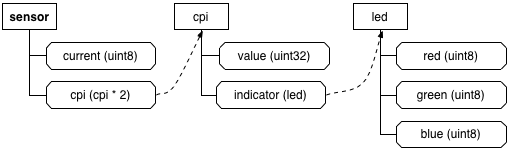
\includegraphics[width=6in]{sensor_nested.png} 
\caption{Nested sensor structure}
\label{fig:sensornested}
\end{figure}

This structure provides the system with information relating to the
fields, types, and nesting. To be usefull for processing json and
generating/interpretting bytearrays, it needs to be flattened with
referneces to other types inlines, arrays expanded, etc. This will
result in the structure shown in Fig.~\ref{fig:sensorflattened}.

\begin{figure}[htbp] %  figure placement: here, top, bottom, or page
   \centering
   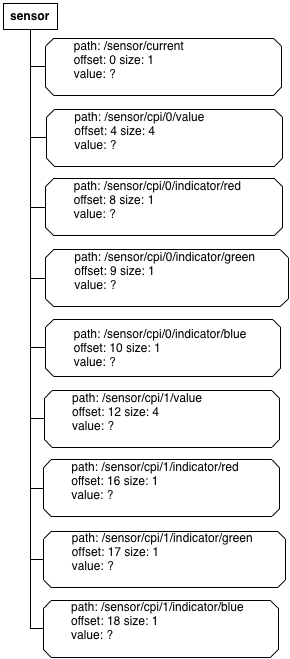
\includegraphics[height=6in]{sensor_flattened.png} 
\caption{Flattened sensor structure}
\label{fig:sensorflattened}
\end{figure}

Here we have each field instantiated, and ordered. Notice the offset
and size bits of data in each field. These are computed based on the
type of each field and relate to the bytearray that will be generated
or torn apart based on this structure. Note that there may be space
between fields in the byte array due to alignment constraints.

The bytearray for our sensor example is shown in
Fig.~\ref{fig:sensorbytearray}.

\begin{figure}[htbp] %  figure placement: here, top, bottom, or page
   \centering
   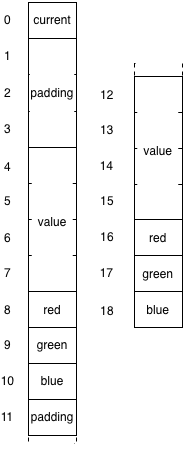
\includegraphics[]{sensor_bytearray.png} 
\caption{Sensor bytearray}
\label{fig:sensorbytearray}
\end{figure}


Also, each field object contains it's path in the original
structure, and also the associated json structure. This is used to
extract the associated data from the json struct when building the
bytearray, as well as place values into the json structure from the
bytearray when getting information from the device.

\bibliographystyle{plain}
\bibliography{lisp}

\end{document}
